\section{Metodologie Agili}

\begin{center}
\textbf{Variabili di controllo nello sviluppo di un processo software}
\end{center}
\paragraph{1.}
\textbf{Tempo}, durata del progetto
\paragraph{2.}
\textbf{Qualità}, soddisfazione degli stakeholders
\paragraph{3.}
\textbf{Risorse}, personale, attrezzatura
\paragraph{4.}
\textbf{Scopo}, cosa c'è da fare, le feature da implementare
\\\\Queste variabili di controllo sono molto difficili da essere controllate tutte insieme, la via più semplice è quella di controllare lo \textbf{scopo}. La \textit{teoria della modellazione del processo software} ha l'obiettivo di controllare le altre variabili.
\begin{center}
\textbf{Modelli per il processo di sviluppo software}
\end{center}
\paragraph{•} 
Cascata (pianificato, lineare)
\paragraph{•}
Spirale (pianificato, iterativo)
\paragraph{•}
Agile (non pianificato, guidato dal test)
\subparagraph{-}
usato solitamente per processi "light"

\subsection{Manifesto Agile}
\begin{center}
\textbf{Metodologie Agili}
\end{center}
C'è un approccio moderno alle pratiche di \textit{sviluppo incrementale}, l'assunzione generale è "La comunicazione è necessariamente imperfetta". Inoltre l'aumento della documentazione non è necessariamente la risposta alle debolezze della pratica in evoluzione dello sviluppo.
\\\\Piuttosto ci sono certe attività complementari (\textbf{best practice} che possono aiutare ad aumentare la qualità o lo scopo delle interazioni come per esempio: 
\subparagraph{•} 
pair programming
\subparagraph{•}
timeboxing
\subparagraph{•}
test-first development

\begin{center}
\textbf{Manifesto Agile}
\end{center}
Ci sono 4 valori dell'Agile e sono: Individui e interazioni, software lavorativo, collaborazione del cliente, rispondere al cambiamento, inoltre il Manifesto Agile segue 12 principi: 
\paragraph{1}
Soddisfazione del cliente
\paragraph{2}
Accettare i cambi richiesti durante lo sviluppo del processo
\paragraph{3}
Consegna frequente del software lavorativo
\paragraph{4}
Collaborazione
\paragraph{5}
Supporto, fiducia, motivazione persone coinvolte
\paragraph{6}
Capacità di interazioni faccia-faccia
\paragraph{7}
il Software lavorativo è la prima misura del progresso
\paragraph{8}
Sviluppo sostenibile
\paragraph{9}
Eccellenza tecnica e un buon design influenzano agilità
\paragraph{10}
Semplicità
\paragraph{11}
Team con auto-organizzazione interna
\paragraph{12}
Auto-miglioramento

\subsection{Processi Agili}
\begin{center}
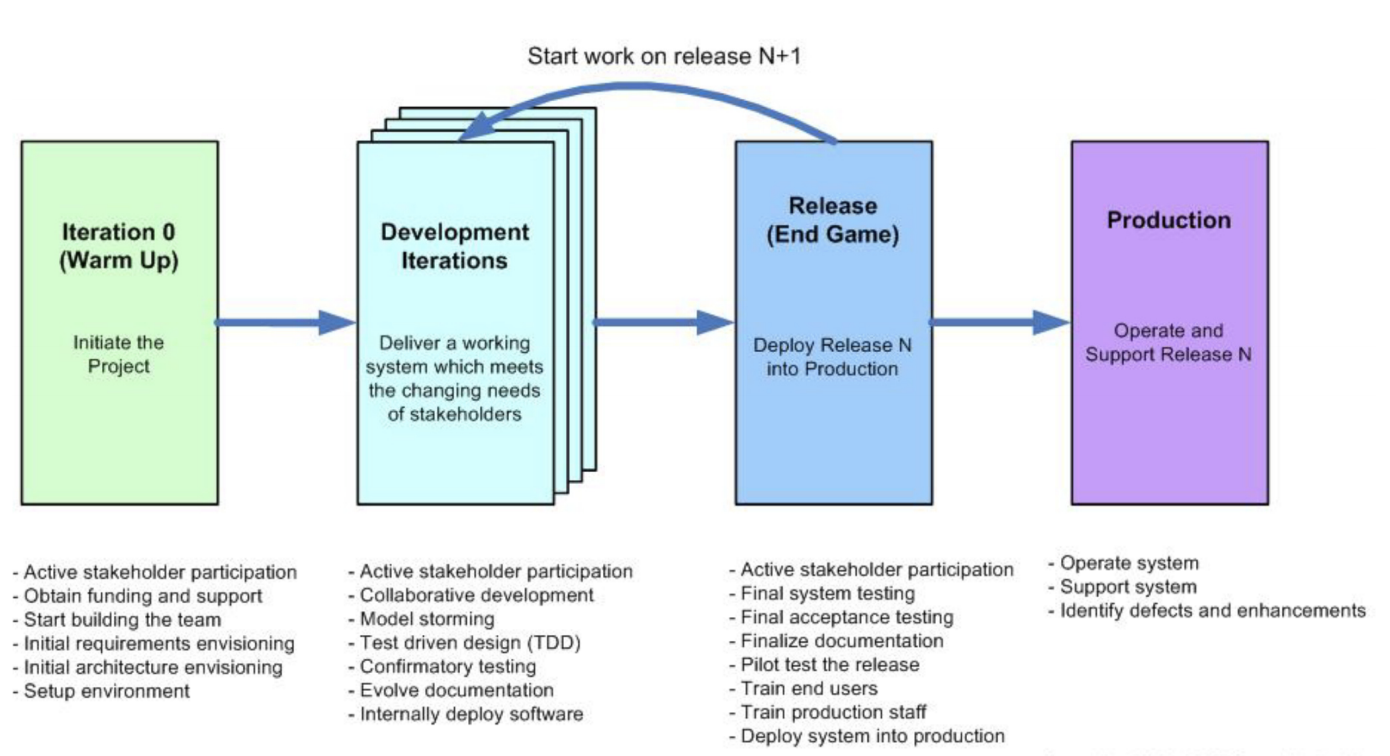
\includegraphics[scale=0.5]{agile1}
\end{center}
Esiste anche l'approccio Extreme Programming (XP), segue uno specifico ciclo di vita che è:$\rightarrow$ \textbf{Planning} $\rightarrow$\textbf{Design}$\rightarrow$\textbf{Programmazione (refactoring)} $\rightarrow$ \textbf{Testing}$\rightarrow$ \textbf{Release}. 
\\Dopo che è stata effettuara una release ed il progetto è andato in produzione si parte a lavorare sulla release N+1.
\\ La consegna continua è data attraverso la pipeline dello sviluppo.
\subsection{Esempio di \textit{best practice} Agile}

Ci sono varie best practice per i metodi agili:
\paragraph{•} 
\begin{flushleft}
\textbf{Planning game}
\end{flushleft}
 Creazione e imporre delle priorità alle User Stories, stimare la difficoltà, selezionare le storie per la nuova release, dividere le storie in compiti, pianificare i compiti per le iterazioni successive. 
\subsection{DevOps}